\subsubsection{Integralfläche berechnen (analytisch)}

\begin{flalign}
    A = \int_{a}^{b}{|f(x) - g(x)|} \,dx \label{eq:Calculate_area}
\end{flalign}

\textcolor{red}{Scale Plot and make a better example}
\begin{center}
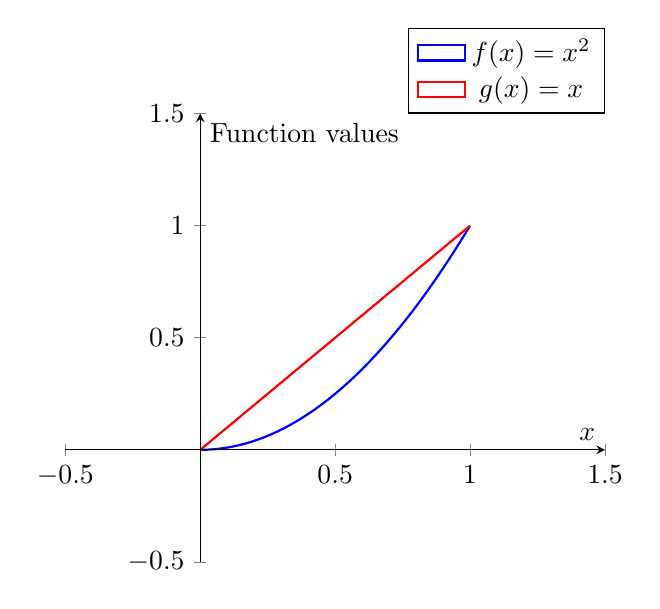
\begin{tikzpicture}
    \begin{axis}[
        axis lines = middle,
        xlabel = \(x\),
        ylabel = {Function values},
        xmin = -0.5, xmax = 1.5,
        ymin = -0.5, ymax = 1.5,
        domain = 0:1,
        samples = 100,
        fill=blue!20,
        area style,
        legend style={at={(1,1)}, anchor=south east},
    ]
    \addplot[blue, thick] {x^2};
    \addplot[red, thick] {x};
    % \addplot[blue!20] fill between[of={x^2}, and={x}]; here is some compiling problem which I couldn't solve at the moment
    \legend{$f(x) = x^2$,$g(x) = x$}
    \end{axis}
\end{tikzpicture}
\end{center}

\subsubsection{Trapezformel (Numerisch)}
\begin{flalign}
    &S_{1} = y_{1} + y_{n} \qquad S_{2} = y_{1} + y_{2} + \dots + y_{n-1}&\notag\\
    &\frac{1}{2} \cdot h \cdot S_{1} + h \cdot S_{2}&\label{eq:Trapezformel}
\end{flalign}
\begin{enumerate}
    \item Stützstellen bestimmen und ausrechnen
    \item Mit Taschenrechner alle Stützstellen mittels Formel \ref{eq:Trapezformel} berechnen 
\end{enumerate}
